\chapter{Shortest Paths}
Ajur was looking at a map of the cemetery map. He was trying to find a way to go to the water fountain. Then he remembered all the discussions he had been having with Rishnak. Ajur told Jura that there may be a method using Graph Theory to find a path and also the shortest path. Rishnak was watching Ajur looking at the map and realized that discussion of path and shortest path (length of the path from source vertex to the destination vertex) would be an ideal topic to pursue next.

Consider a graph\footnote{In the case of spanning trees, we consider only undirected graphs; however shortest paths, we can consider both undirected and directed graphs.}. Rishnak asked Ajur to find the shortest path from a specified source vertex to a specified destination vertex. Consider the following Graph shown in Figure \ref{12g1}
\begin{figure}
\begin{center}
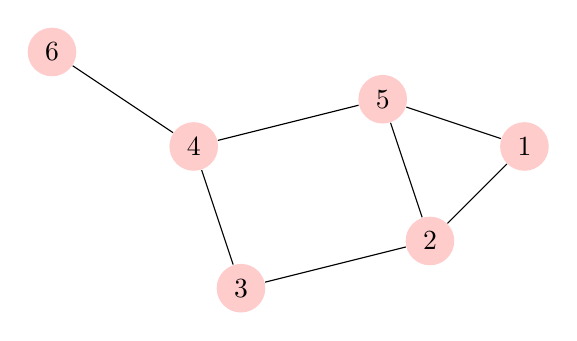
\begin{tikzpicture}
  [scale=.6,auto=left,every node/.style={circle,fill=red!20}]
  \node (n6) at (1,10) {6};
  \node (n4) at (4,8)  {4};
  \node (n5) at (8,9)  {5};
  \node (n1) at (11,8) {1};
  \node (n2) at (9,6)  {2};
  \node (n3) at (5,5)  {3};

  \foreach \from/\to in {n6/n4,n4/n5,n5/n1,n1/n2,n2/n5,n2/n3,n3/n4}
    \draw (\from) -- (\to);

\end{tikzpicture}
\caption{ Example Graph, We want to find the shortest path from vertex 1 to vertex 6}\label{12g1}
\end{center}
\end{figure}

Ajur jumped up and down with excitement and said he could draw the shortest path from source vertex (1) to destination vertex (6). Rishnak asked him to draw the graph. Ajur drew the following graph \ref{12g2}

\begin{figure}
\begin{center}
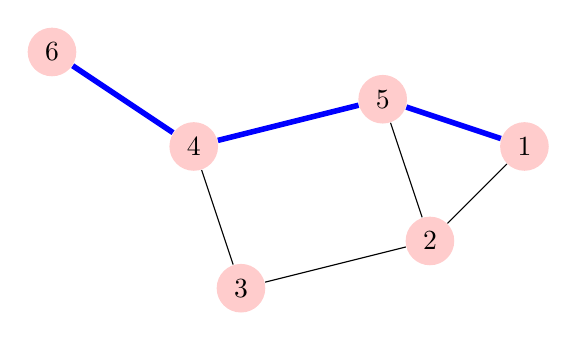
\begin{tikzpicture}
  [scale=.6,auto=left,every node/.style={circle,fill=red!20}]
  \node (n6) at (1,10) {6};
  \node (n4) at (4,8)  {4};
  \node (n5) at (8,9)  {5};
  \node (n1) at (11,8) {1};
  \node (n2) at (9,6)  {2};
  \node (n3) at (5,5)  {3};

  \foreach \from/\to in {n6/n4,n4/n5,n5/n1}
    \draw [line width=2 pt,color=blue] (\from) -- (\to);
\foreach \from/\to in {n3/n4,n3/n2,n2/n1,n2/n5}
    \draw  (\from) -- (\to);

\end{tikzpicture}
\caption{ Example Graph, Shortest Path (of length 3) from vertex 1 to vertex 6 in Graph \ref{12g1} - shortest path is drawn in thick lines.}\label{12g2}
\end{center}
\end{figure}

Rishnak admired Ajur's enthusiasm but wanted to find out whether one can find a general methof of finding the shortest path from a source vertex to a destination vertex.